
\providecommand{\Cat}{\mathcal{C}at}
\providecommand{\sSet}{s\mathcal{S}et}

\section{\trEnrichedCategory{}与富集函子}\label{sec:enriched-categories-and-enriched-functors}

现在我们短暂地切换视角，先解释名词短语「\trEnrichedCategory」的含义，然后再
讨论把一个通常的 1-\trCategory{}「富集」起来需要些什么。从本节起直到 A.6 节，
我们固定一个\trComplete{}且\trCocomplete{}的\trCartesianClosed{}\trCategory{}
$(\mathcal{V},\times,1)$ 作为富集所用的基。

\begin{definition}\label{def:enriched-category}
一个 \textbf{$\mathcal{V}$-富集范畴}（$\mathcal{V}$-enriched category）或%
\textbf{$\mathcal{V}$-范畴}（$\mathcal{V}$-category）$\mathcal{C}$ 由如下数据
给出：
\begin{itemize}
\item 对象的一个汇集；%
\item 对每对对象 $x,y\in\mathcal{C}$，一个 \textbf{hom-对象}（hom-object）
  $\mathcal{C}(x,y)\in\mathcal{V}$；
\item 对每个 $x\in\mathcal{C}$，一个指定的 \textbf{单位元}（identity
  element），由映射 $\mathrm{id}_{x}\colon 1\to\mathcal{C}(x,x)\in\mathcal{V}$
  编码；并且对每个 $x,y,z\in\mathcal{C}$，一个指定的 \textbf{复合映射}
  （composition map）
  $\circ\colon\mathcal{C}(y,z)\times\mathcal{C}(x,y)\to\mathcal{C}(x,z)\in\mathcal{V}$，
  其满足结合性与单位这两组条件，两个交换图表均居于
  $\mathcal{V}$ 之中。\footnote{这些图表省去了涉及乘积\trBifunctor{} $\times$
  及其单位对象 $1$ 的那些结合性与单位自然\trIsomorphism。在一个%
  \trCartesianClosed{}\trCategory{}中，这些自然\trIsomorphism{}是
  \emph{典范的}——而非作为额外数据给出；在更一般的\emph{封闭对称幺半范畴}的
  情形中它们则作为额外数据给出（见\cref{ex:closed-symmetric-monoidal}）。}
\end{itemize}
\begin{center}
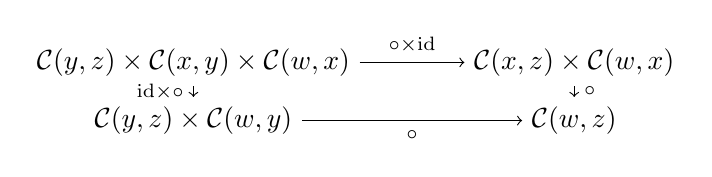
\begin{tikzpicture}[x=1.6em,y=1.5em]
  \node (tl) at (0,1.4)
    {$\mathcal{C}(y,z)\times\mathcal{C}(x,y)\times\mathcal{C}(w,x)$};
  \node (tr) at (8.6,1.4) {$\mathcal{C}(x,z)\times\mathcal{C}(w,x)$};
  \node (bl) at (0,0) {$\mathcal{C}(y,z)\times\mathcal{C}(w,y)$};
  \node (br) at (8.6,0) {$\mathcal{C}(w,z)$};
  \draw[->] (tl) -- node[above]{$\scriptstyle\circ\times\mathrm{id}$} (tr);
  \draw[->] (tl) -- node[left]{$\scriptstyle\mathrm{id}\times\circ$} (bl);
  \draw[->] (tr) -- node[right]{$\scriptstyle\circ$} (br);
  \draw[->] (bl) -- node[below]{$\scriptstyle\circ$} (br);
\end{tikzpicture}

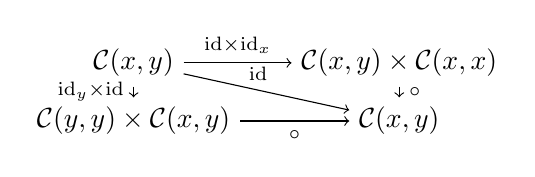
\begin{tikzpicture}[x=1.6em,y=1.5em]
  \node (tl) at (0,1.4) {$\mathcal{C}(x,y)$};
  \node (tr) at (6.0,1.4) {$\mathcal{C}(x,y)\times\mathcal{C}(x,x)$};
  \node (bl) at (0,0) {$\mathcal{C}(y,y)\times\mathcal{C}(x,y)$};
  \node (br) at (6.0,0) {$\mathcal{C}(x,y)$};
  \draw[->] (tl) -- node[above]{$\scriptstyle\mathrm{id}\times\mathrm{id}_{x}$} (tr);
  \draw[->] (tl) -- node[left]{$\scriptstyle\mathrm{id}_{y}\times\mathrm{id}$} (bl);
  \draw[->] (tl) -- node[above,pos=0.45]{$\scriptstyle\mathrm{id}$} (br);
  \draw[->] (tr) -- node[right]{$\scriptstyle\circ$} (br);
  \draw[->] (bl) -- node[below]{$\scriptstyle\circ$} (br);
\end{tikzpicture}
\end{center}
\end{definition}

显然，由\eqref{eq:assoc-unit-squares}的图表可见，一个局部小的 1-\trCategory{}定义了一个富集于
$\mathcal{S}et$ 之上的\trCategory。\cref{def:underlying-set-functor}的底集
函子可用来定义一个富集\trCategory{}的「底范畴」。

\begin{definition}\label{def:underlying-category}
若 $\mathcal{C}$ 是一个 $\mathcal{V}$-范畴，其 \textbf{底范畴}（underlying
category）$\mathcal{C}_{0}$ 是具有相同对象之集的 1-\trCategory，其 hom-集由把
底集函子 $(-)_{0}\colon\mathcal{V}\to\mathcal{S}et$ 施于诸 hom-对象
$\mathcal{C}(x,y)\in\mathcal{V}$ 上而定义。在多数情形下，我们对 hom-对象与
hom-集均写作「$\mathcal{C}(x,y)$」并以措辞来消歧，但必要时
「$\mathcal{C}(x,y)_{0}$」也是底范畴之 hom-集的一种常用记法。
\end{definition}

注意：$\mathcal{V}$-范畴的恒等箭头 $\mathrm{id}_{x}\colon 1\to\mathcal{C}(x,x)$
按定义是 hom-集 $\mathcal{C}(x,x)_{0}:=\mathcal{V}(1,\mathcal{C}(x,x))$ 的一个%
\trElement。底范畴中两支箭头 $f\colon 1\to\mathcal{C}(x,y)$ 与
$g\colon 1\to\mathcal{C}(y,z)$ 的复合，定义为如下复合所构造出的那支箭头
\[ 1\xrightarrow{\ g\times f\ }\mathcal{C}(y,z)\times\mathcal{C}(x,y)
   \xrightarrow{\ \circ\ }\mathcal{C}(x,z) \]

与围绕\cref{def:underlying-set-functor}的讨论相类比，当人们谈及把一个先验非
富集的\trCategory{} $\mathcal{C}$ 「富集」于 $\mathcal{V}$ 之上时，任务便是
定义一个如\cref{def:enriched-category}中的 $\mathcal{V}$-富集范畴，使其底范畴
恢复出 $\mathcal{C}$。当 $\mathcal{V}=\Cat$ 时，任务是定义一个 2-\trCategory，
使其底 1-\trCategory{}即为所给者。当 $\mathcal{V}=\sSet$ 时，任务是定义诸
$n$-箭头的单纯 hom-集，使得 0-箭头即为所给者。当一个%
\trSimpliciallyEnrichedCategory{} $\mathcal{C}$ 如第 1 章中的%
\cref{dig:simplicial-categories}所解释的那样被
编码为 $\Cat$ 中的一个\trSimplicialObject{} $\mathcal{C}_{\bullet}$ 时，其底
范畴便是\trCategory{} $\mathcal{C}_{0}$，这进一步佐证了%
\cref{def:underlying-category}中引入的概念。

例如，\cref{def:cartesian-closed}中那样的一个\trCartesianClosed{}\trCategory{}
$\mathcal{V}$ 可被富集而定义出一个 $\mathcal{V}$-范畴。

\begin{lemma}\label{lem:cartesian-closed-v-category}
一个\trCartesianClosed{}\trCategory{} $\mathcal{V}$ 定义一个 $\mathcal{V}$-范畴，
其：
\begin{itemize}
\item 对象为 $\mathcal{V}$ 的对象；
\item 居于 $\mathcal{V}$ 中、从 $a$ 到 $b$ 的 hom-对象是\trInternalHom{}
  $b^{a}$；
\item 恒等映射 $\mathrm{id}_{a}\colon 1\to a^{a}$ 与复合映射
  $\circ\colon c^{b}\times b^{a}\to c^{a}$ 定义为
  \[ 1\times a\simeq a \qquad\text{以及}\qquad
     c^{b}\times b^{a}\times a
     \xrightarrow{\ \mathrm{id}\times\mathrm{ev}\ }c^{b}\times b
     \xrightarrow{\ \mathrm{ev}\ }c \]
  的转置，后者使用笛卡尔封闭伴随的余单位 $\mathrm{ev}$ 来定义。
\end{itemize}
\end{lemma}

\begin{proof}
任务是验证\cref{def:enriched-category}中的两个交换图表在 $\mathcal{V}$ 中
成立，然后观察到\cref{lem:underlying-set-of-internal-hom}揭示了：由本陈述所
定义的 $\mathcal{V}$-范畴的底范畴正是 1-\trCategory{} $\mathcal{V}$。我们把
恒等条件留给读者，在此验证结合性。

把复合映射定义为伴随转置，这蕴涵它的伴随转置——即下方的右上复合——由左下
复合给出：
\begin{rveq}\label{eq:composition-transpose-square}
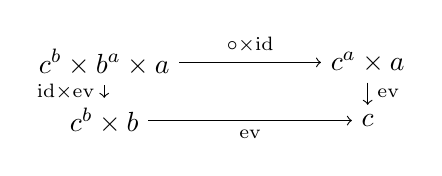
\begin{tikzpicture}[x=1.7em,y=1.5em]
  \node (tl) at (0,1.4) {$c^{b}\times b^{a}\times a$};
  \node (tr) at (5.6,1.4) {$c^{a}\times a$};
  \node (bl) at (0,0) {$c^{b}\times b$};
  \node (br) at (5.6,0) {$c$};
  \draw[->] (tl) -- node[above]{$\scriptstyle\circ\times\mathrm{id}$} (tr);
  \draw[->] (tl) -- node[left]{$\scriptstyle\mathrm{id}\times\mathrm{ev}$} (bl);
  \draw[->] (tr) -- node[right]{$\scriptstyle\mathrm{ev}$} (br);
  \draw[->] (bl) -- node[below]{$\scriptstyle\mathrm{ev}$} (br);
\end{tikzpicture}
\end{rveq}
下左侧的结合性图表交换，当且仅当下右侧作为外边界复合出现的那张转置后的图表
交换：
\begin{center}
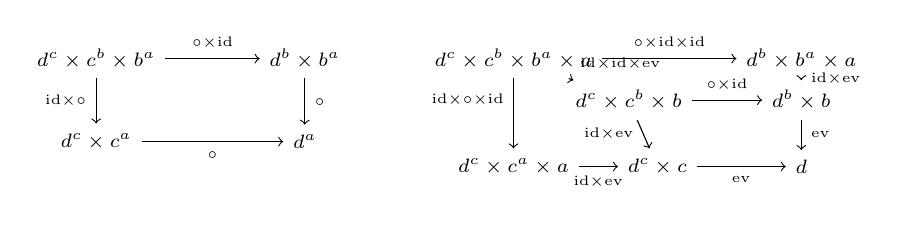
\begin{tikzpicture}[x=1.3em,y=1.5em,every node/.style={font=\scriptsize}]
  \node (LTL) at (0,2.9) {$d^{c}\times c^{b}\times b^{a}$};
  \node (LTR) at (5.8,2.9) {$d^{b}\times b^{a}$};
  \node (LBL) at (0,0.9) {$d^{c}\times c^{a}$};
  \node (LBR) at (5.8,0.9) {$d^{a}$};
  \draw[->] (LTL) -- node[above]{$\scriptstyle\circ\times\mathrm{id}$} (LTR);
  \draw[->] (LTL) -- node[left]{$\scriptstyle\mathrm{id}\times\circ$} (LBL);
  \draw[->] (LTR) -- node[right]{$\scriptstyle\circ$} (LBR);
  \draw[->] (LBL) -- node[below]{$\scriptstyle\circ$} (LBR);
  \node at (7.9,1.9) {$\rightsquigarrow$};
  \node (T)  at (11.6,2.9) {$d^{c}\times c^{b}\times b^{a}\times a$};
  \node (TR) at (19.6,2.9) {$d^{b}\times b^{a}\times a$};
  \node (IL) at (14.8,1.9) {$d^{c}\times c^{b}\times b$};
  \node (IR) at (19.6,1.9) {$d^{b}\times b$};
  \node (BL) at (11.6,0.3) {$d^{c}\times c^{a}\times a$};
  \node (BM) at (15.6,0.3) {$d^{c}\times c$};
  \node (BR) at (19.6,0.3) {$d$};
  \draw[->] (T) -- node[above]{$\scriptstyle\circ\times\mathrm{id}\times\mathrm{id}$} (TR);
  \draw[->] (T) -- node[left,pos=0.3]{$\scriptstyle\mathrm{id}\times\circ\times\mathrm{id}$} (BL);
  \draw[->] (T) -- node[above right,pos=0.35]{$\scriptstyle\mathrm{id}\times\mathrm{id}\times\mathrm{ev}$} (IL);
  \draw[->] (IL) -- node[above]{$\scriptstyle\circ\times\mathrm{id}$} (IR);
  \draw[->] (IL) -- node[left,pos=0.5]{$\scriptstyle\mathrm{id}\times\mathrm{ev}$} (BM);
  \draw[->] (TR) -- node[right]{$\scriptstyle\mathrm{id}\times\mathrm{ev}$} (IR);
  \draw[->] (IR) -- node[right]{$\scriptstyle\mathrm{ev}$} (BR);
  \draw[->] (BL) -- node[below]{$\scriptstyle\mathrm{id}\times\mathrm{ev}$} (BM);
  \draw[->] (BM) -- node[below]{$\scriptstyle\mathrm{ev}$} (BR);
\end{tikzpicture}
\end{center}
这由 $\times$ 的二函子性以及上方交换方块的两个实例推得。
\end{proof}

\begin{definition}\label{def:free-v-category}
1-\trCategory{} $\mathcal{C}$ 上的 \textbf{自由 $\mathcal{V}$-范畴}（free
$\mathcal{V}$-category）具有与之相同的对象之集，其 hom-对象定义为以 hom-集
$\mathcal{C}(x,y)$ 标引的\trTerminal{}对象 $1\in\mathcal{V}$ 的余积
$\coprod_{\mathcal{C}(x,y)}1$。恒等映射
$\mathrm{id}_{x}\colon 1\to\coprod_{\mathcal{C}(x,x)}1$ 由以恒等箭头标引的那个
分量的包含给出，复合映射则通过让复合函数作用于诸标引集来定义：
\[ \coprod_{\mathcal{C}(y,z)}1\times\coprod_{\mathcal{C}(x,y)}1
   \cong\coprod_{\mathcal{C}(y,z)\times\mathcal{C}(x,y)}1
   \xrightarrow{\ \coprod\circ\ }\coprod_{\mathcal{C}(x,z)}1 \]
\end{definition}

例如，自由 $\Cat$-富集范畴是没有非恒等 2-\trCell{}的那些，而自由
$\sSet$-富集范畴则是在正维数中没有非退化箭头的那些。我们对 1-\trCategory{}
$\mathcal{C}$ 与它所生成的自由 $\mathcal{V}$-范畴使用相同的记号，并以措辞来
消歧。

\begin{definition}\label{def:v-enriched-functor}
一个 \textbf{$\mathcal{V}$-富集函子}（$\mathcal{V}$-enriched functor）或
\textbf{$\mathcal{V}$-函子}（$\mathcal{V}$-functor）
$F\colon\mathcal{C}\to\mathcal{D}$ 由如下数据给出：
\begin{itemize}
\item 对象上的一个映射，把每个 $x\in\mathcal{C}$ 送到某个 $Fx\in\mathcal{D}$；
\item 对每对对象 $x,y\in\mathcal{C}$，hom-对象上的一个内部作用，由态射
  $F_{x,y}\colon\mathcal{C}(x,y)\to\mathcal{D}(Fx,Fy)\in\mathcal{V}$ 给出，
  使得 $\mathcal{V}$-函子性图表交换：
\end{itemize}
\begin{center}
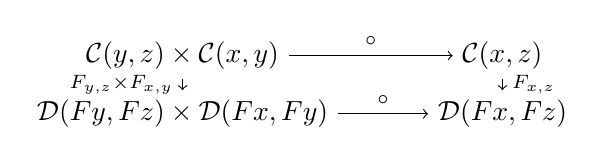
\begin{tikzpicture}[x=1.7em,y=1.5em]
  \node (tl) at (0,1.4) {$\mathcal{C}(y,z)\times\mathcal{C}(x,y)$};
  \node (tr) at (6.8,1.4) {$\mathcal{C}(x,z)$};
  \node (bl) at (0,0) {$\mathcal{D}(Fy,Fz)\times\mathcal{D}(Fx,Fy)$};
  \node (br) at (6.8,0) {$\mathcal{D}(Fx,Fz)$};
  \draw[->] (tl) -- node[above]{$\scriptstyle\circ$} (tr);
  \draw[->] (tl) -- node[left]{$\scriptstyle F_{y,z}\times F_{x,y}$} (bl);
  \draw[->] (tr) -- node[right]{$\scriptstyle F_{x,z}$} (br);
  \draw[->] (bl) -- node[above]{$\scriptstyle\circ$} (br);
\end{tikzpicture}
\qquad
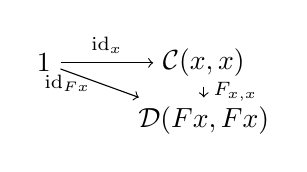
\begin{tikzpicture}[x=1.7em,y=1.5em]
  \node (t)  at (0,1.4) {$1$};
  \node (tr) at (3.4,1.4) {$\mathcal{C}(x,x)$};
  \node (b)  at (3.4,0) {$\mathcal{D}(Fx,Fx)$};
  \draw[->] (t) -- node[above]{$\scriptstyle\mathrm{id}_{x}$} (tr);
  \draw[->] (tr) -- node[right]{$\scriptstyle F_{x,x}$} (b);
  \draw[->] (t) -- node[left]{$\scriptstyle\mathrm{id}_{Fx}$} (b);
\end{tikzpicture}
\end{center}
\end{definition}

一个原型性的例子由可表示函子给出：

\begin{example}\label{exa:enriched-representable}
对任何 $\mathcal{V}$-范畴 $\mathcal{C}$ 与对象 $c\in\mathcal{C}$，\textbf{富集
可表示 $\mathcal{V}$-函子}（enriched representable $\mathcal{V}$-functor）
$\mathcal{C}(c,-)\colon\mathcal{C}\to\mathcal{V}$ 在对象上由指定
$x\in\mathcal{C}\mapsto\mathcal{C}(c,x)\in\mathcal{V}$ 来定义，其在 hom-对象上
的内部作用则定义为 $\mathcal{C}$ 的内部复合映射的伴随转置：
\[ \mathcal{C}(x,y)\xrightarrow{\ \mathcal{C}(c,-)_{x,y}\ }
   \mathcal{C}(c,y)^{\mathcal{C}(c,x)}
   \;\rightsquigarrow\;
   \mathcal{C}(x,y)\times\mathcal{C}(c,x)\xrightarrow{\ \circ\ }
   \mathcal{C}(c,y) \]
$\mathcal{V}$-函子性图表是 $\mathcal{C}$ 中结合性与恒等图表的转置。反变的富集
可表示函子类似地定义（见\cref{ex:opposite-v-category}）。
\end{example}

\begin{remark}\label{rem:two-step-enrichment}
一个富集可表示函子可以被视为相应的非富集可表示函子的一种「两步」富集：第一步
把 hom-集富集为 $\mathcal{V}$ 中的 hom-对象，第二步把复合函数富集为
$\mathcal{V}$ 中的一个内部复合映射。把一个 1-\trCategory{} $\mathcal{C}$ 富集
成一个以 $\mathcal{C}$ 为其底 1-\trCategory{}的 $\mathcal{V}$-范畴，所需者
多于 hom 二函子的一个单纯的\trLifting：
\begin{center}
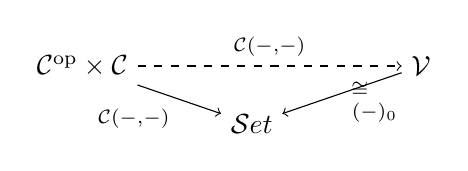
\begin{tikzpicture}[x=1.7em,y=1.4em]
  \node (tl) at (0,1.5) {$\mathcal{C}^{\mathrm{op}}\times\mathcal{C}$};
  \node (tr) at (7.2,1.5) {$\mathcal{V}$};
  \node (b)  at (3.6,0) {$\mathcal{S}et$};
  \draw[->,dashed] (tl) -- node[above]{$\scriptstyle\mathcal{C}(-,-)$} (tr);
  \draw[->] (tl) -- node[below left]{$\scriptstyle\mathcal{C}(-,-)$} (b);
  \draw[->] (tr) -- node[below right]{$\scriptstyle(-)_{0}$} (b);
  \node at (5.9,0.9) {$\scriptstyle\cong$};
\end{tikzpicture}
\end{center}
此外，取值于 $\mathcal{V}$ 中的可表示函子
$\mathcal{C}(-,-)\colon\mathcal{C}^{\mathrm{op}}\times\mathcal{C}\to\mathcal{V}$
必须是\cref{ex:v-bifunctor}意义下的一个 $\mathcal{V}$-二函子，这告诉我们：
复合映射可以在 $\mathcal{V}$ 内部定义，而且恒等定律与结合定律也在那里成立。
\end{remark}

「取底非富集范畴」与「取自由范畴」这两种构造都是函子式的（见%
\cref{ex:underlying-free-functorial}）。这两种构造之间的关系由下述命题概括，
其证明留作练习，因为它被\cref{cor:underlying-free-2-adjunction}所加强。

\begin{proposition}\label{prop:free-v-category-fully-faithful}
自由 $\mathcal{V}$-范畴函子定义底范畴函子的一个\trFullyFaithful{}
\trLeftAdjoint。从而，一个 $\mathcal{V}$-范畴是自由的，恰当时它经由该伴随的
余单位\trIsomorphism{}于其底范畴上的自由范畴。
\end{proposition}

\begin{proof}
\cref{ex:proof-free-v-category-fully-faithful}。
\end{proof}

\subsection*{练习}

\begin{exercise}\label{ex:underlying-category-is-category}
验证\cref{def:underlying-category}所描述的富集范畴之底范畴确实是一个%
\trCategory。
\end{exercise}

\begin{exercise}\label{ex:unit-condition}
验证\cref{lem:cartesian-closed-v-category}之证明中留给读者的那个单位条件。
\end{exercise}

\begin{exercise}\label{ex:opposite-v-category}
定义一个 $\mathcal{V}$-范畴的 \textbf{反者}（opposite），并对偶化%
\cref{exa:enriched-representable}以定义反变的富集可表示函子。
\end{exercise}

\begin{exercise}\label{ex:v-bifunctor}
\begin{enumerate}[label=(\roman*)]
\item 定义两个 $\mathcal{V}$-范畴的 \textbf{笛卡尔积}（cartesian product）。
\item 定义一个 \textbf{多变量 $\mathcal{V}$-函子}（multivariable
  $\mathcal{V}$-functor）。
\item 利用这些概念证明：任何 $\mathcal{V}$-范畴 $\mathcal{C}$ 都配备有一个%
  \trCanonical{} $\mathcal{V}$-二函子
  $\mathcal{C}(-,-)\colon\allowbreak\mathcal{C}^{\mathrm{op}}\times\allowbreak\mathcal{C}\to\allowbreak\mathcal{V}$，
  它限制到协变与反变的可表示函子上。
\end{enumerate}
\end{exercise}

\begin{exercise}\label{ex:underlying-free-functorial}
\begin{enumerate}[label=(\roman*)]
\item 定义一个富集函子的底函子。
\item 证明从富集函子到底非富集函子的过渡是函子式的。
\item 定义一个非富集函子上的自由富集函子。
\item 证明从非富集函子到自由富集函子的过渡是函子式的。
\end{enumerate}
\end{exercise}

\begin{exercise}[A.7.6]\label{ex:proof-free-v-category-fully-faithful}
证明\cref{prop:free-v-category-fully-faithful}。
\end{exercise}

